\section{Dynamic Structural Graph Operations}
\label{sec:eval:dynamic}

% TODO: Update spider chart — merge Insert Tput / Update Tput into a single
% "Ingest/Update" axis and add a "Dynamic OLAP" axis (geomean or sum of
% BFS+PR+WCC on graph500-26).

Dynamic graph processing systems target high-performance
ingest and operate primarily in memory.
We use three such systems to establish a baseline:
Teseo~\cite{teseo2021deLeo}, LiveGraph~\cite{zhu2019livegraph}, and
GraphOne~\cite{graphone2019kumar}.
Each achieves high ingest throughput through lightweight write paths:
GraphOne appends edges to a lock-free ring buffer drained by a background archiver; Teseo uses optimistic latching on fat-tree segments; LiveGraph maintains a transactional edge log backed by mmap.
No system requires a read-optimized replica for analytics.
GraphOne's background archiver pre-builds per-vertex adjacency lists in a read store; analytics merge these with unarchived edges into flat per-vertex arrays without per-edge version checks.
LiveGraph iterates its mmap'd per-vertex edge blocks under snapshot isolation, filtering each entry with two epoch-based timestamp comparisons.
Teseo scans its sorted fat-tree segments sequentially; clean segments skip version checks, dirty ones consult a sparse undo log. 
 

Most dynamic graph systems have no way to persist data across restarts; the exceptions are LiveGraph, which supports file-backed mmap, and GraphOne, which provides a write-ahead log.
For a fair comparison with Teseo, we disable persistence in LiveGraph and GraphOne, so all three baselines operate under comparable in-memory conditions.
Recall that \project{} is inherently persistent; to best approximate in-memory behavior in the presence of updates, we disable the write-ahead log and checkpointing and size WiredTiger's cache to prevent most evictions.
We do not take advantage of WiredTiger's in-memory mode, because it would be contrary to our design objective.
As a result, we avoid as much disk I/O as possible, but do not turn off the persistence machinery entirely.
Specifically, \project{} maintains the graph in WiredTiger's persistable, page-oriented B-tree format at all times, which involves byte-comparable key serialization, disk-block-granular page geometry, page-image reconciliation, extent/block management, and an always-on eviction subsystem. 
This machinery consumes CPU on the ingest path: not the cost of persisting data, but of maintaining a structure that is persistable by construction.
GraphOne and LiveGraph decouple durability from their in-memory representation and pay essentially nothing for the option.
However, such designs have consequences, e.g., GraphOne does not enforce transactional consistency during updates. 
GraphOne delegates duplicate checking to the caller; its snapshot mechanism is too heavyweight to invoke per-edge, and throughput collapses  if used that way.
Teseo, provides transactional semantics comparable to \project{}, it has  no durable representation and incurs no persistence overhead.
LiveGraph has similar transactional semantics, but since it relies on mmap, the host OS can evict pages at any time, so the write ordering needed for consistency and crash recovery are difficult, if not impossible, to guarantee. 

We conduct four experiments:
(1)~a scalability study that varies writer thread count,
(2)~an insertion benchmark at each system's optimal thread count,
(3)~a sustained mixed insert-and-delete workload that replays a graph
update log,
(4)~a graph analytics benchmark (PageRank, BFS, and weakly connected components) run after finishing the insertion.

%%%%%%%%%%%%%%%%%%%%%%%%%%%%%%%%%%%%%%%%%%%%%%%%%%%%%%%%%%%%%%%%%%%%%%%%%%%%%%%%
% TODO: regenerate as a single-column, single-panel figure (scalability only;
% drop the peak-throughput bar chart — those numbers are now in the prose).
\begin{figure*}[ht]
  \centering
  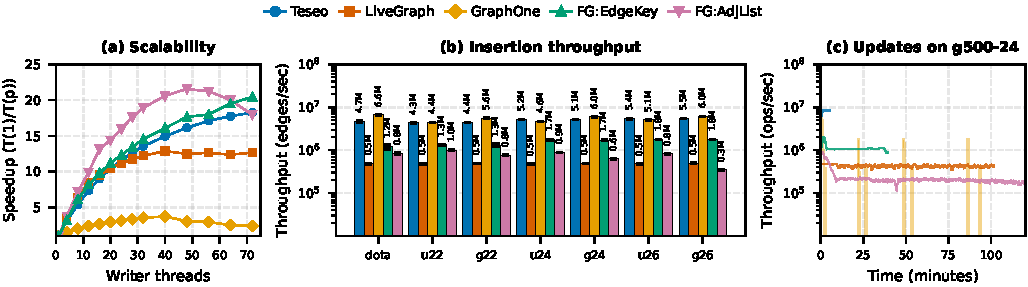
\includegraphics[width=\textwidth]{fig/dynamic/dynamic_triptych_ts2.pdf}
  \caption{Dynamic graph operations: (a)~insertion scalability: scalability with increasing writer thread count on graph500-24, (b)~peak insertion throughput across datasets, (c)~update (insert/delete workload) throughput on graph500-24.}
  \label{fig:dynamic-scaling}
\end{figure*}
%%%%%%%%%%%%%%%%%%%%%%%%%%%%%%%%%%%%%%%%%%%%%%%%%%%%%%%%%%%%%%%%%%%%%%%%%%%%%%%%

\section{Insertion Scalability}

We insert the edges of graph500-24 while varying the number of writer threads from 1 to 72 to identify each system's optimal concurrency (\autoref{fig:dynamic-scaling}a).
GraphOne peaks at 6.3\,M~edges/s with 40~threads but degrades beyond that point as cross-socket contention on its single ring buffer increases.
Teseo scales the most consistently, reaching 5.1\,M~edges/s at 72~threads with no sign of saturation.
LiveGraph plateaus near 0.49\,M~edges/s at 32--40~threads.
\project{} EdgeKey reaches 1.7\,M~edges/s at 72~threads; Adjacency List peaks at 0.77\,M~edges/s with 48~threads.
Based on these results, we fix GraphOne and LiveGraph at 40~threads and Teseo and both \project{} configurations at 72~threads for all subsequent experiments.

\section{Ingest and Update Throughput}

Having identified optimal thread counts, we next examine ingest and sustained update performance.
\autoref{fig:dynamic-scaling}b reports insertion-only throughput across six datasets (51\,M to 1.05\,B edges).
GraphOne and Teseo dominate, sustaining 5.6--6.6 and 4.3--5.5\,M~edges/s respectively, 3 to 5$\times$ faster than \project{} EdgeKey (1.2--1.8\,M~edges/s).
This gap reflects the "persistence machinery tax" in \project{} even when no logging, checkpointing, or evictions occur.
GraphOne does blind-writes and does not do any existence checks during inserts; both GraphOne and LiveGraph use append-only paths.
\project{} EdgeKey is $3\times$ faster than LiveGraph (0.48\,M~edges/s).

Under a sustained mixed workload (2.6\,B operations, ${\sim}$55\% insertions and ${\sim}$45\% deletions on graph500-24), the picture changes.
Teseo sustains 7.0\,M~ops/s, which is $\approx$30\% higher than its insertion-only rate, and can be attributed to updates creating space for new insertions in an update-in-place data structure such as the Teseo tree.
More specifically, as De Leo et al. noted in their paper, updates trigger fewer rebalances and leaf splits\cite{teseo2021deLeo}.
However, GraphOne, despite leading the insertion benchmark, collapses to 0.05 \, M~ops/s, a 115$\times$ drop.
The root cause is deletions: GraphOne's background archiver must locate the target edge to set a tombstone, and its append-only layout has no index for this lookup; on power-law graphs the resulting linear scan stalls the archiver and back-pressures writers.
\project{} EdgeKey sustains 1.06\,M~ops/s, and LiveGraph sustains 0.42\,M~ops/s.
In LiveGraph, both edge additions and deletions are bottlenecked on finding the edge; the actual mutation is an append or a timestamp flip respectively. 
Vertex deletions simply tombstone the vertex block: incident edges are left in place and reclaimed by background compaction.
\project{}, by contrast, performs immediate cleanup: every incident edge is removed in a single transaction. 
Under the Adjacency List layout, this requires rewriting each affected neighbor's packed list; under SplitEdgeKey, each edge is an independent B-tree row, so removal is a point delete.

\project{}'s two layouts present a clear tradeoff.
EdgeKey stores one B-tree row per edge; inserts are independent, carry no read-modify-write overhead, and incur essentially zero transaction aborts, scaling monotonically to 72~threads.
Adjacency List stores one record per vertex, so every edge insert appends to the source vertex's record.
Under power-law degree distributions, concurrent writers issue conflicting modifications to the records of high-degree vertices, producing a high rollback rate that caps throughput at ${\sim}$48 threads and ${\sim}$0.8\,M~edges/s.

\section{Post-Ingestion Analytics}
We next examine how well each system performs after ingest on graph analytic workloads.
After completing insertion, we run BFS, PageRank~(PR), and weakly connected components~(WCC) in parallel across all physical cores; no updates run during the analytics phase.
The results are in \autoref{tab:analytics-main}.
Recall that, at this point, the in-memory baselines hold the graph only as a transient structure that will be lost if the system shuts down or crashes; there are no redundant copies, no durable snapshots.

% \textbf{Excluding the cold open.}
% % Unlike the purely in-memory baselines, \project{} stores the graph in WiredTiger. 
% In \project{}, immediately after ingestion, data resides as dirty pages in the buffer cache.
% To ensure that graphalytics kernels run on a stable, consistent, read-only view of the graph, \project{} forces a checkpoint and opens a set of per-thread read-only handles before the first kernel runs.
% The checkpoint makes the first run expensive: it triggers
% \emph{reconciliation}, in which WiredTiger walks every dirty page and reconciles
% its in-memory updates into the page images that constitute the queryable snapshot.
% Since the first Graphalytics kernel invocation triggers the checkpoint, the first run on a freshly built graph includes this one-time cost (varies from 59s on graph500-22 to 26 minutes on graph500-26).
% Because subsequent kernels amortize it, we report steady-state time.
% % \project{}'s checkpoint time is, however, far from negligible and grows with graph size: the forced checkpoint takes 59\,s and 68\,s on the SF-22 graphs, roughly five minutes on SF-24 (298\,s / 284\,s), and about 26--27\,min on the billion-edge SF-26 graphs (1536\,s / 1628\,s); opening the read-only handles adds at most 16\,s. 
% % The competing systems incur no comparable cost, because they require no reconciliation step: LiveGraph's first run is within noise of its warm runs, and Teseo adds only a few seconds of cache warm-up.
% The cold open is therefore the price FlexoGraph pays \emph{once} to convert a write-optimized store into a consistent read snapshot that subsequently serves analytics at in-memory speed.

\project{} Adjacency List is the only system that delivers fast, stable performance across all three kernels and both graph families.
Teseo runs BFS fastest (0.61\,s on graph500-26) but its PageRank and WCC degrade sharply at scale---27\,s and 12\,s respectively---while \project{}'s PageRank stays at 5.7\,s, $4.7\times$ faster.
LiveGraph is competitive on uniform WCC (0.95\,s) but scales poorly on power-law inputs.
GraphOne presents the starkest read-write contrast: despite being the fastest inserter, its WCC collapses at graph500-26 and is over $30\times$ slower than every other system, while its BFS and PageRank remain comparable to LiveGraph and Teseo.
The ingest-optimized EdgeKey layout, is orders of magnitude slower on analytics (640\,s for BFS on g500-24 versus 0.37\,s for AdjList), confirms that layout choice is the dominant factor in analytical performance.

\textbf{Takeaway.}
Not having a separate high-speed ingest path costs \project{} 3--5$\times$ on raw insertion relative to purpose-built in-memory systems, an expected and acceptable penalty.
This cost does not carry over to analytics, where \project{} Adjacency List matches or outperforms every baseline across all kernels and scales, while retaining the ability to persist and recover the graph that none of the in-memory systems provide.